
%% Макрос для введения. Совместим со старым стилевиком.
\startprefacepage

В последнее время количество информации во всем мире стремительно увеличивается. 
Согласно \cite{two-times} за каждые два года суммарное количество данных в интернете увеличивается в два раза. 
Аналогичные результаты подтверждаются исследованиями, которые были проведены автором во время работы в компании ВКонтакте. 
Эта компания владеет одноименным сайтом, на котором пользователи могут обмениваться сообщениями. 
На рис.~\ref{fig1} показано количество сообщений, отправленных пользователями в течении разных месяцев. 
Эти данные заставили задуматься о пересмотре архитектуры хранения сообщений, а также улучшении эффективности их обработки.

\begin{figure}[h!]
  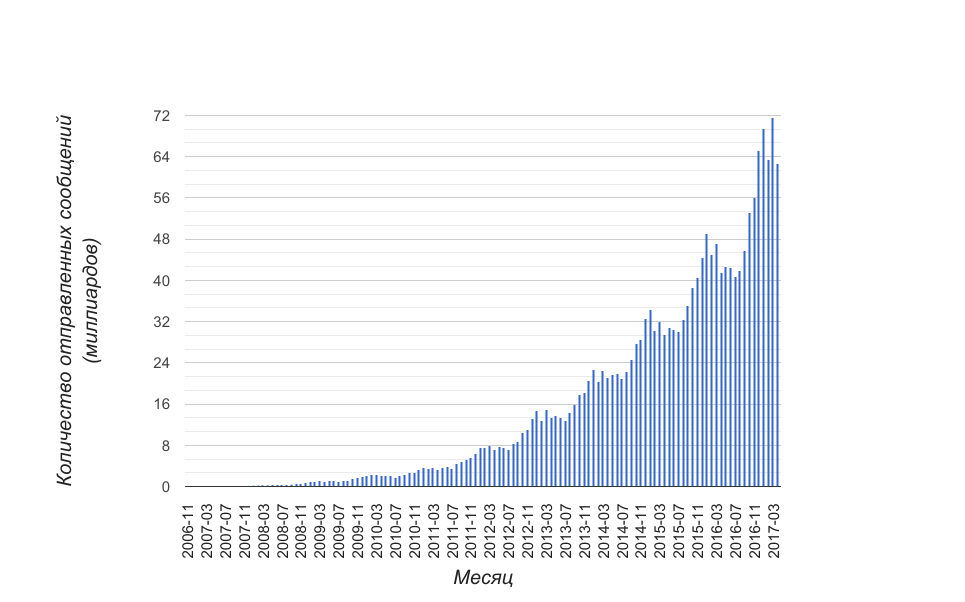
\includegraphics[width=\linewidth]{pics/msgs-num.png}
  \caption{Количество отправляемых сообщений}
  \label{fig1}
\end{figure}

Конечной целью улучшения способа хранения пользовательских сообщений является уменьшение количества серверов,
 на которых работает сервис, а также улучшение качества его работы. К последнему в основном относится скорость 
 работы. Интересует как средняя скорость ответа на запросы, так и, например, ответ на вопрос <<какая часть 
 запросов выполняется дольше секунды>>. Забегая вперед, хочется сказать, что все эти показатели удалось 
 существенно улучшить, уменьшив при этом количество используемых серверов в два раза.

Одним из способов оптимизации хранения сообщений является их сжатие. Оно позволяет уменьшить количество 
занимаемого места в несколько раз. Однако, сервис обмена сообщениями должен предоставлять пользователю возможность
 прочитать любое свое сообщение, а также уметь искать по ним, что накладывает некоторые ограничения на алгоритмы, которые можно использовать для сжатия.
Существует огромное количество алгоритмов сжатия данных без потерь. История их создания начинается в 
середине прошлого века \cite{kudryashov}. 

Интересным примером того, как хорошо сейчас умеют сжимать данные является 
\cite{compression-banchmark}. Участникам соревнования предлагается написать алгоритм сжатия первого 
миллиарда символов xml-версии английской Википедии. На текущий момент лучший алгоритм смог сжать исходные 
данные в 8,29 раза. Это действительно впечатляющий результат, однако, таких коэффициентов сжатия сложно 
добиться в реальных задачах. Проблема связана как со спецификой данных (в исходных данных для соревнования
 много xml-сущностей, которые хорошо сжимаются), так и в ресурсах, которые необходимы алгоритму. Так для
  сжатия гигабайта Википедии алгоритм-победитель использовал больше недели процессорного времени и 27
   дополнительных гигабайт оперативной памяти.

Проблема применения существующих алгоритмов для сжатия сообщений пользователей в том, что необходимо либо
 сжимать каждое сообщение отдельно, либо уметь разархивировать произвольный кусок данных. В первом случае 
 большинство алгоритмов сжатия теряют свою эффективность из-за маленького размера сообщений. А алгоритмы,
  которые могут разжимать произвольный кусок данных достаточно эффективно, автору работы не известны.

В данной работе рассмотрены различные способы сжатия текстовых сообщений короткой длины, а также представлен 
новый способ, основанный на алгоритме Хаффмана.